\chapter{Related Work and Background}
\label{ch:background}

This chapter defines the two ingredients shared by every experiment in the thesis: the microscopic particle simulator (Section~\ref{sec:collective_motion}) and the KDE coarse-graining operator that maps discrete trajectories to the smooth macroscopic fields consumed by both the EF-ROM and WSINDy branches (Section~\ref{subsec:kde} and its multi-field extension in Section~\ref{sec:multifield_cg}).  The coarse-graining step is not mere preprocessing; it is a modeling choice that determines which physical structures are visible at the field level and therefore which effective mechanisms can be identified or forecast.

\section{Collective motion models}
\label{sec:collective_motion}

This section defines the microscopic simulator that generates all training
and test data.  The model extends the discrete-time
Vicsek alignment framework studied in~\cite{alvarez2025eqfree} with Morse
attraction--repulsion forces~\cite{dorsogna2006morse} and variable-speed dynamics, producing a family
of regimes whose macroscopic behavior ranges from gentle drift to
near-singular collapse.  Each microscopic ingredient---alignment,
attraction--repulsion, and speed mode---motivates a specific candidate term in the WSINDy library (Chapter~\ref{ch:wsindy_methodology}): alignment maps to self-advection and relaxation terms, Morse forces to nonlocal density-weighted gradients, and variable speed to flux--density coupling that the present library does not close.

\subsection{Vicsek-style noisy alignment}

The alignment rule is the minimal ingredient shared by every regime in the
benchmark and gives rise to the self-advection and relaxation terms in the
WSINDy momentum library.
We consider a discrete-time Vicsek-type alignment model for self-driven agents. At discrete times
$t_n=n\Delta t$, agent $i$ has position $x_i^n\in\Omega\subset\mathbb{R}^2$ and unit heading
$p_i^n := (\cos\theta_i^n,\ \sin\theta_i^n)\in\mathbb{S}^1$, with constant-speed velocity $v_i^n=v_0\,p_i^n$ for a fixed $v_0>0$.
Given an interaction radius $R>0$, the neighbor set is $\mathcal{N}_i^n := \{\, j\in\{1,\dots,N\} : d_\Omega(x_i^n,x_j^n) \le R \,\}$, where $d_\Omega$ denotes the domain distance. The local mean heading direction is obtained by averaging neighbors' headings and renormalizing:
\[
s_i^n := \sum_{j\in\mathcal{N}_i^n} p_j^n,
\qquad
\bar p_i^n :=
\begin{cases}
s_i^n/\|s_i^n\|, & \|s_i^n\|>\varepsilon,\\
p_i^n, & \text{otherwise},
\end{cases}
\]
with a small $\varepsilon>0$ to avoid division by zero.
\noindent Equivalently, one may write $\bar\theta_i^n=\mathrm{Arg}(\bar p_i^n)=\mathrm{atan2}((\bar p_i^n)_2,(\bar p_i^n)_1)$ and update angles modulo $2\pi$. The noisy Vicsek update rotates the mean direction by an angular perturbation $\Delta\theta_i^n$:
\begin{equation}
p_i^{n+1} = R(\Delta\theta_i^n)\,\bar p_i^n,
\qquad
R(\phi)=
\begin{pmatrix}
\cos\phi & -\sin\phi\\
\sin\phi & \cos\phi
\end{pmatrix},
\label{eq:vicsek_heading_vec}
\end{equation}
followed by the forward Euler position update
\begin{equation}
x_i^{n+1} = x_i^n + \Delta t\,v_0\,p_i^{n+1}.
\label{eq:vicsek_position}
\end{equation}
This is the standard Vicsek alignment mechanism~\cite{vicsek1995vicsek}; its mean-field limit and the continuum equations that arise from it are studied in~\cite{toner2005hydrodynamics,bertin2006boltzmann,degond2008continuum}.
The noise model is specified per regime (uniform or Gaussian angular noise); the original model uses uniform angular noise
$\Delta\theta_i^n \sim \mathrm{Unif}(-\eta/2,\ \eta/2)$ with strength $\eta$; in addition, we also consider Gaussian noise
$\Delta\theta_i^n \sim \mathcal{N}(0,\sigma^2)$.
When variances are matched, $\sigma = \eta/\sqrt{12}$.
The nature of the order--disorder transition can depend on whether scalar (intrinsic) or vectorial (extrinsic) noise is used~\cite{gregoirechate2004}.

% ============================================================
% Boundary conditions + attraction--repulsion with fixed speed
% ============================================================

\subsection{Boundary conditions}
\label{sec:boundary_conditions}

We consider a rectangular domain $\Omega = [0,L_x)\times[0,L_y)$
with periodic boundary conditions throughout this thesis.
Distances are computed via the standard minimal-image convention,
and periodicity is enforced componentwise after each position update:
$x_{i,\alpha}^{n+1} \leftarrow x_{i,\alpha}^{n+1} \bmod L_\alpha$
for $\alpha\in\{1,2\}$.

% ----------------------------
% Morse attraction--repulsion
% ----------------------------
\subsection{Attraction--repulsion interactions with Morse potentials}
\label{sec:morse_forces}

Beyond pure alignment, we incorporate short-range repulsion and
longer-range attraction via a Morse-type interaction
force~\cite{dorsogna2006morse}.
Let $r_{ij} := x_i - x_j$, $r := \|r_{ij}\|$, and
$\hat r_{ij} := r_{ij}/r$.  The radial Morse force magnitude is
\begin{equation}
f(r)
=
\frac{C_r}{\ell_r} e^{-r/\ell_r}
-
\frac{C_a}{\ell_a} e^{-r/\ell_a},
\label{eq:morse_fr}
\end{equation}
where $C_r,C_a>0$ denote repulsion and attraction strengths and
$\ell_r,\ell_a>0$ their interaction lengths.
The pairwise force is
$F_{ij} = f(\|x_i-x_j\|)\,\hat r_{ij}$,
summed over neighbours within a cutoff radius
$r_{\mathrm{cut}} = 5\,\max(\ell_r,\ell_a)$.
A cohesive regime is obtained when $\ell_r<\ell_a$ (short-range
repulsion, longer-range attraction).

\emph{Constant-speed mechanism.}\;
Morse forces steer headings without changing speed:
\begin{equation}
\tilde p_i^n
=
\bar p_i^n
+
\mu_t\,\frac{F_i^n}{\|F_i^n\|+\varepsilon},
\qquad
p_i^{n+1}
=
\frac{\tilde p_i^n}{\|\tilde p_i^n\|},
\qquad
v_i^{n+1}
=
v_0\,p_i^{n+1},
\label{eq:direction_only_force_update}
\end{equation}
where $\mu_t$ is the translational mobility.
This yields clean latent dynamics while producing milling,
clustering, and ring formation~\cite{bhaskar2019topology}.

\emph{Variable-speed dynamics (this thesis).}\;
As a stress test for the ROM pipeline, we extend the Morse mechanism to allow force-driven dynamics with variable speed:
$v_i(t+\Delta t) = v_i(t) + \Delta t\,\mu_t\,F_i(t)$,
$x_i(t+\Delta t) = x_i(t) + \Delta t\,v_i(t+\Delta t)$.
When speed is no longer slaved to heading, the effective
phase-space dimension increases and the POD latent coordinates
may no longer capture the dynamics faithfully---making VS regimes
a stress test for low-dimensional ROM assumptions.
The full update pseudocode is given in Algorithm~\ref{alg:vicsek}
(Appendix~\ref{app:detailed_algorithms}); the key step is the sequential
application of alignment averaging, force steering, noise injection, and
position update on the periodic torus.

\begin{figure}[htbp]
\centering
\makebox[\textwidth][c]{%
\begin{tabular}{@{}c@{\;}c@{\;}c@{}}
  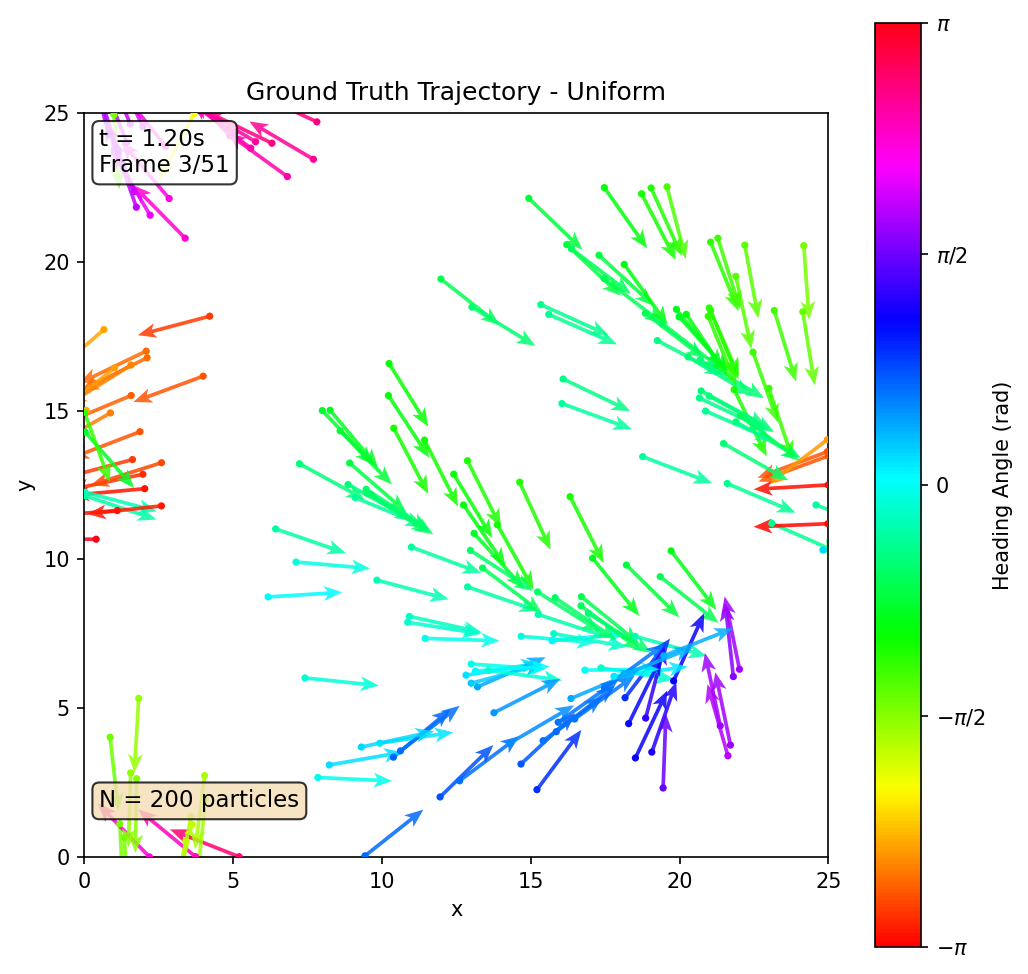
\includegraphics[width=0.33\textwidth]{ch3_experimentation/figures/traj_DYN1_t0.png} &
  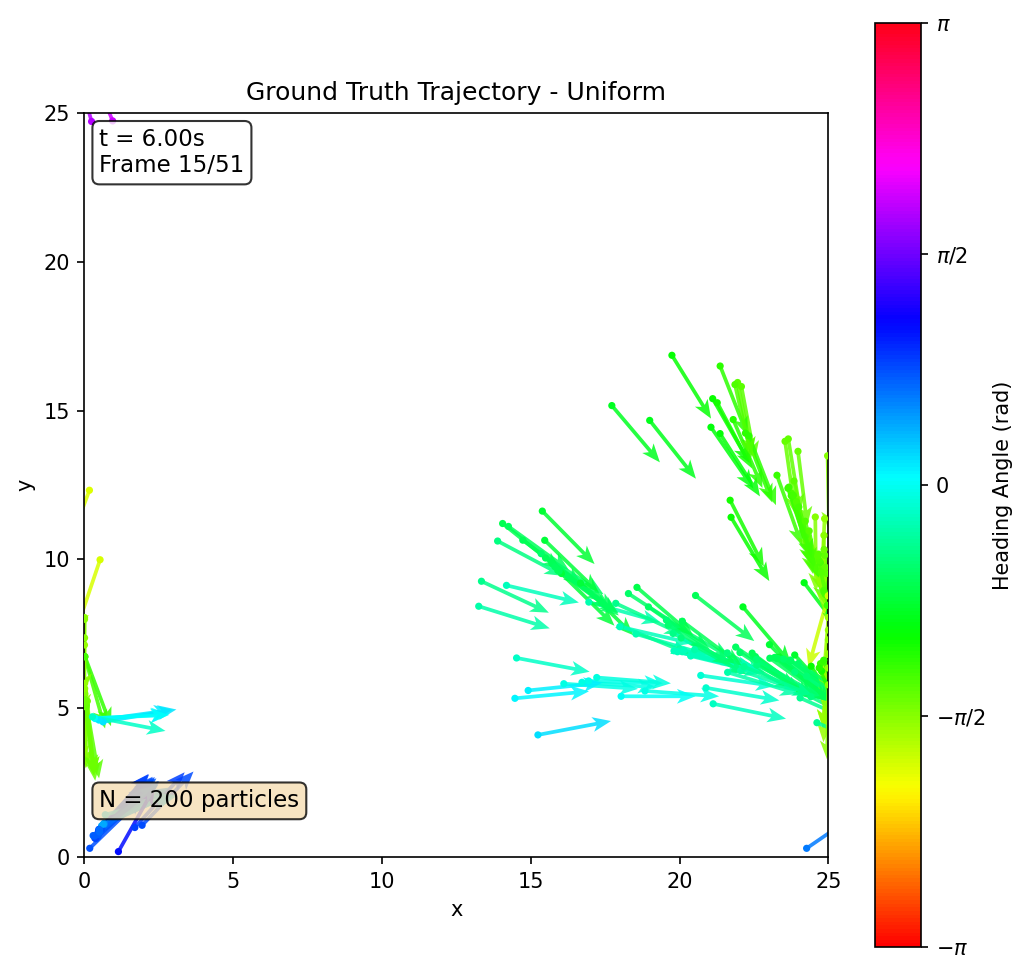
\includegraphics[width=0.33\textwidth]{ch3_experimentation/figures/traj_DYN1_t15.png} &
  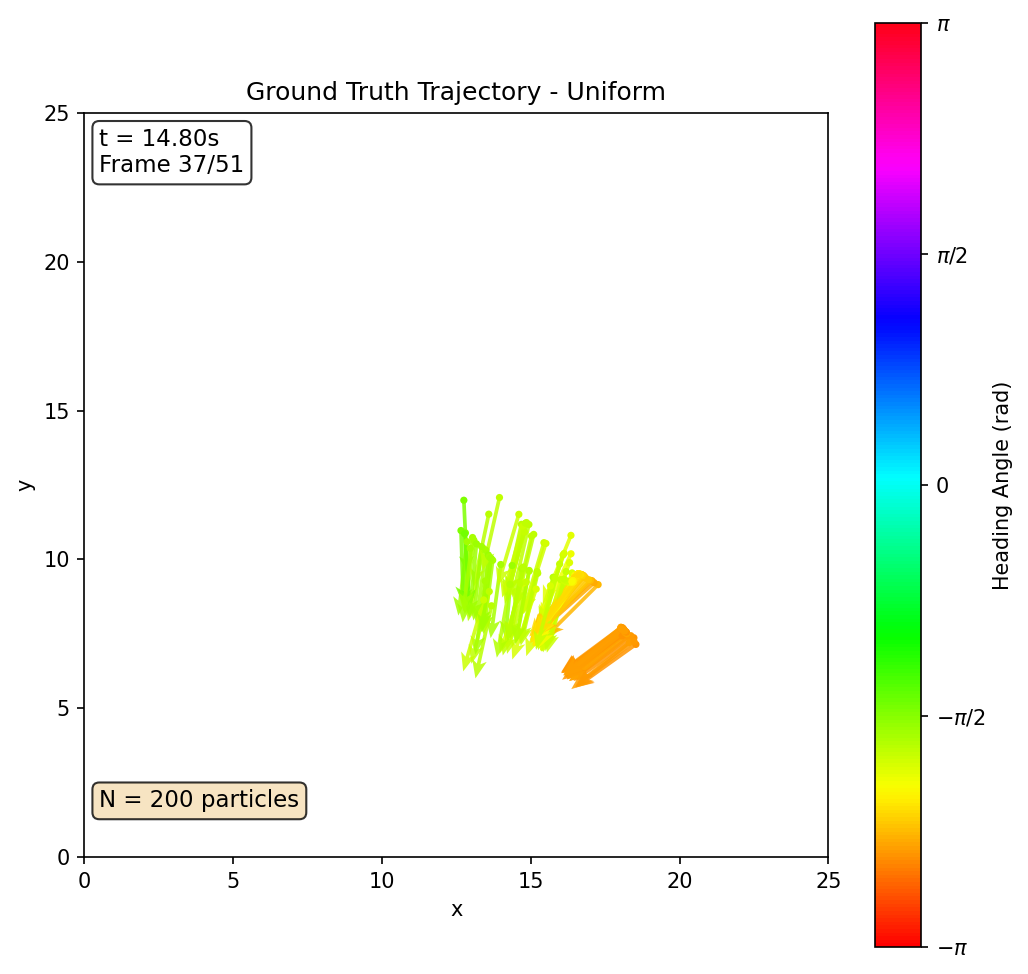
\includegraphics[width=0.33\textwidth]{ch3_experimentation/figures/traj_DYN1_t38.png} \\[-4pt]
  \multicolumn{3}{c}{\small (a) Gentle crawl regime (weak Morse forces, low speed)} \\[2pt]

  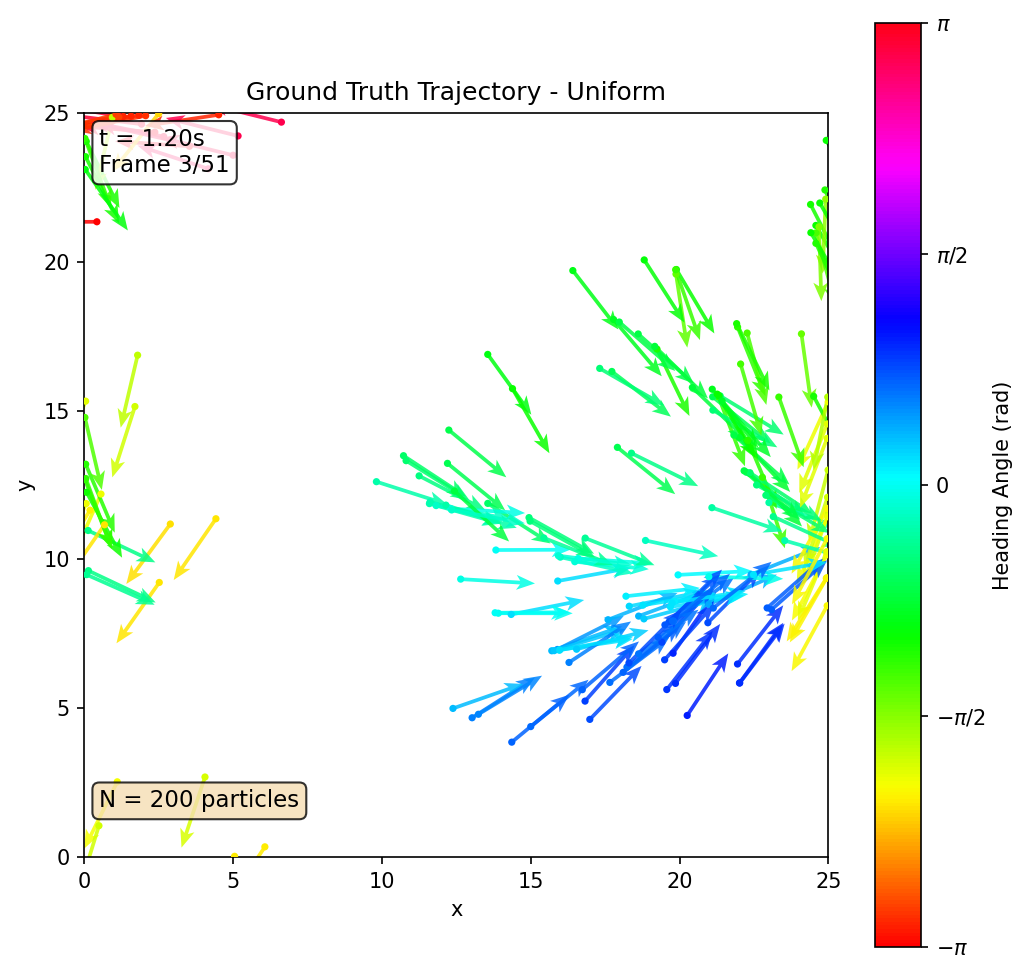
\includegraphics[width=0.33\textwidth]{ch3_experimentation/figures/traj_DYN4_t0.png} &
  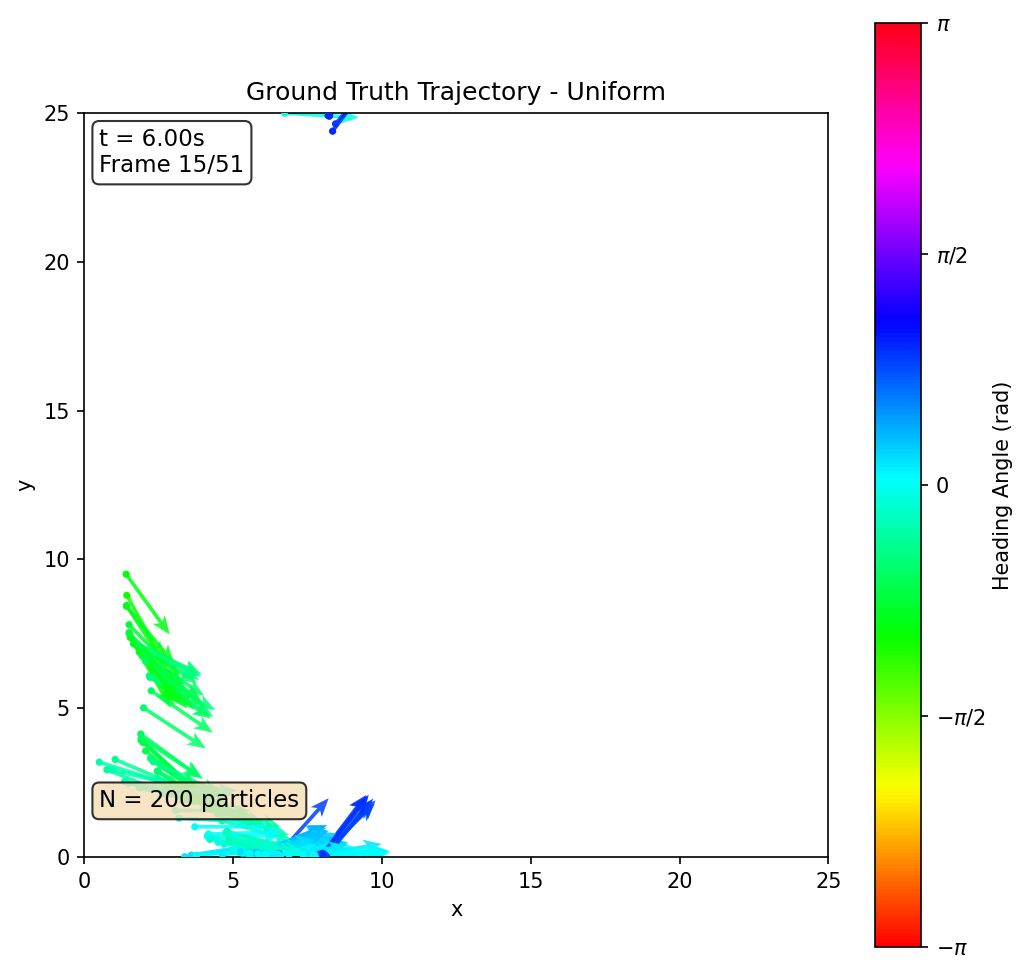
\includegraphics[width=0.33\textwidth]{ch3_experimentation/figures/traj_DYN4_t15.png} &
  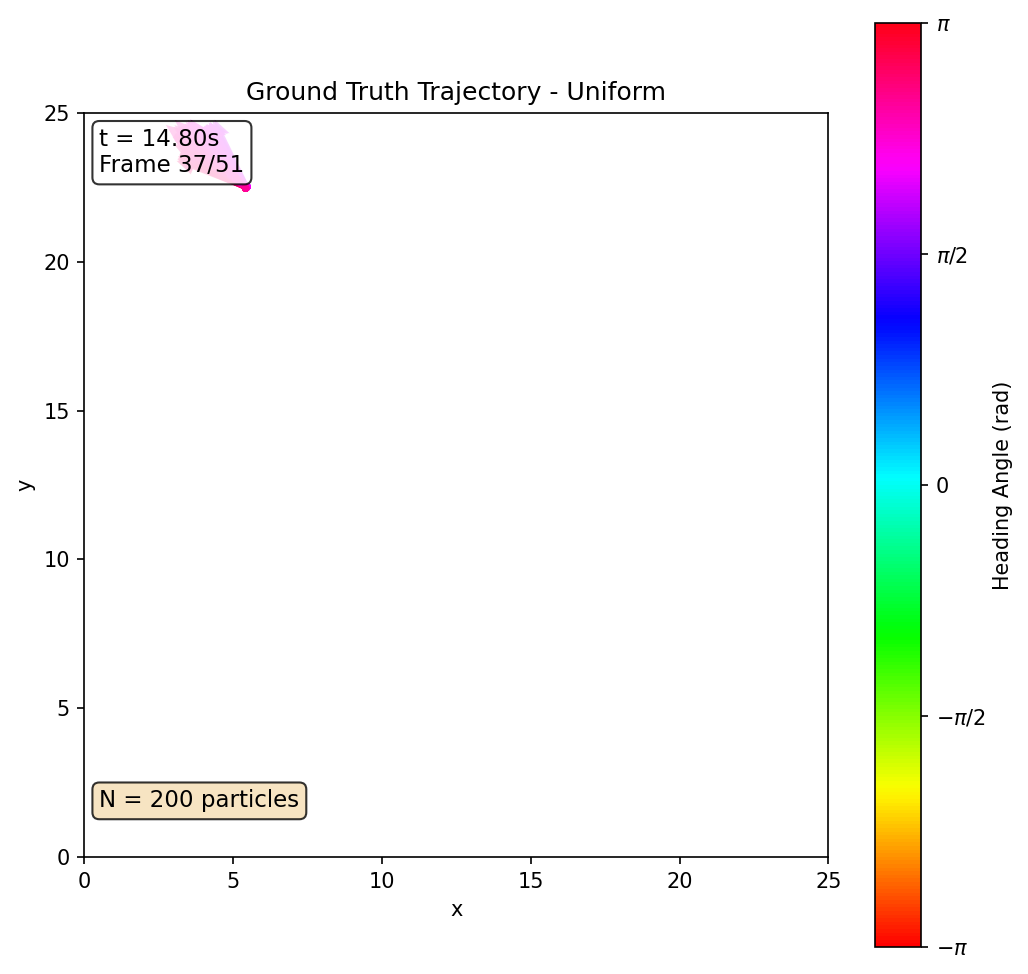
\includegraphics[width=0.33\textwidth]{ch3_experimentation/figures/traj_DYN4_t38.png} \\[-4pt]
  \multicolumn{3}{c}{\small (b) Blackhole regime (strong attraction, near-singular collapse)} \\[2pt]

  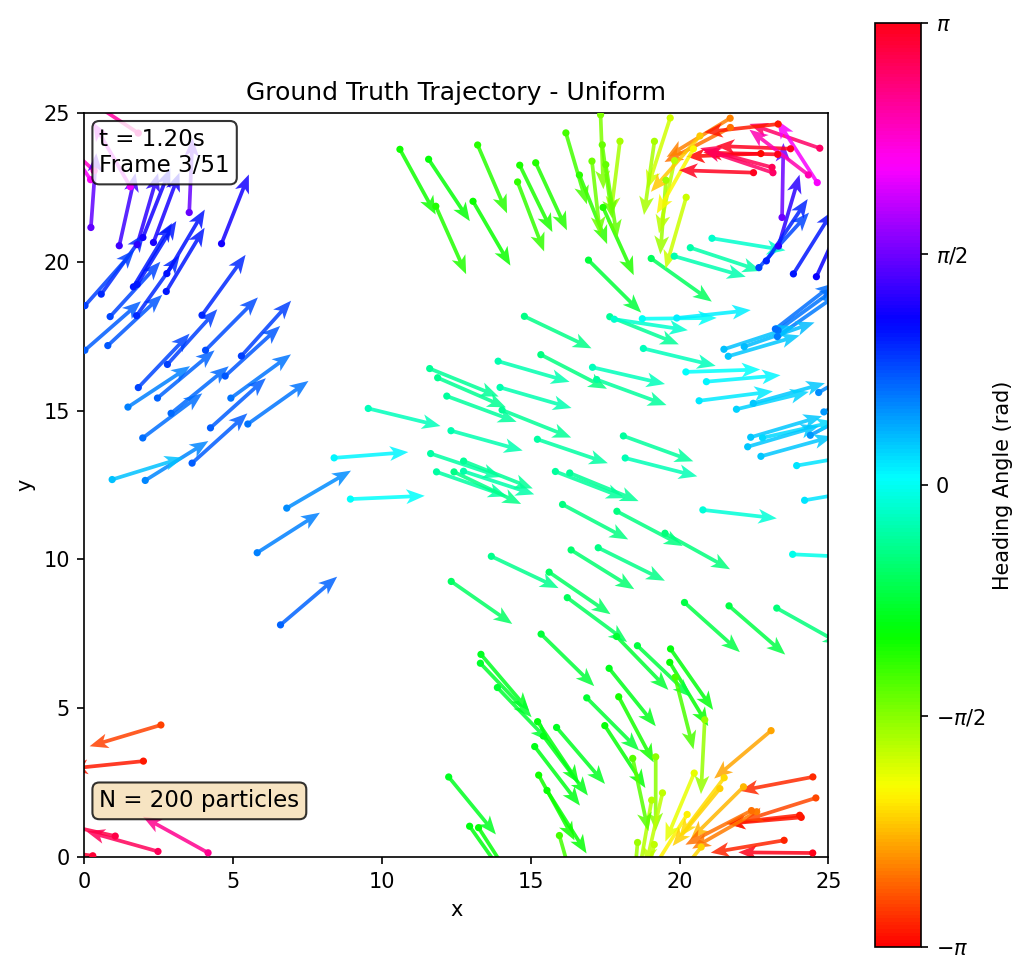
\includegraphics[width=0.33\textwidth]{ch3_experimentation/figures/traj_DYN7_t0.png} &
  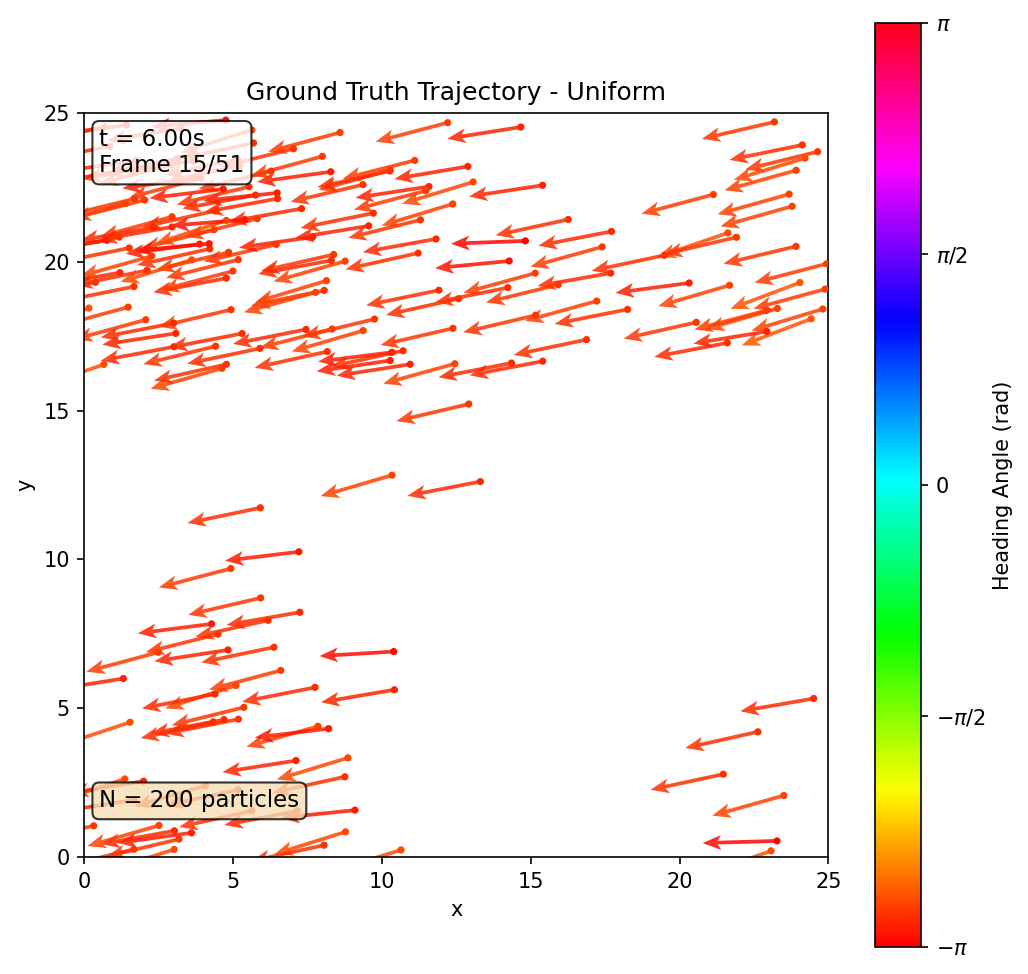
\includegraphics[width=0.33\textwidth]{ch3_experimentation/figures/traj_DYN7_t15.png} &
  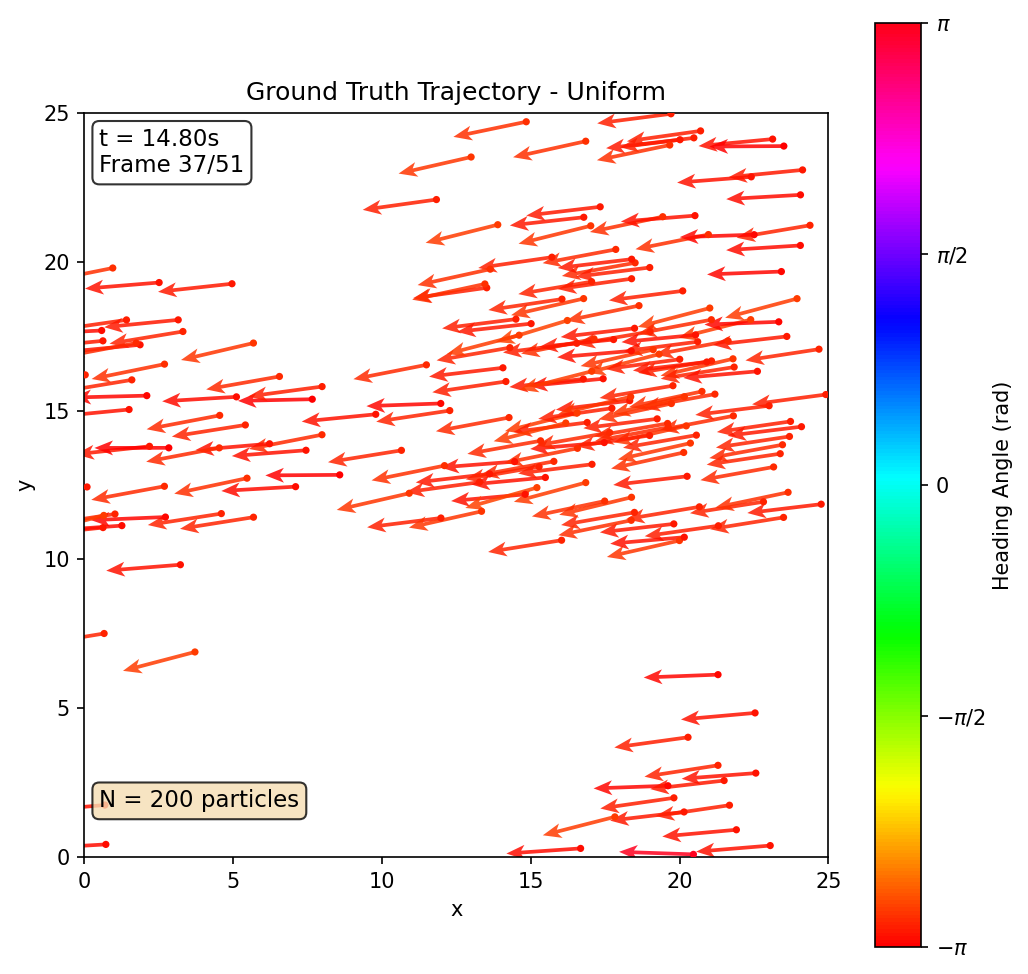
\includegraphics[width=0.33\textwidth]{ch3_experimentation/figures/traj_DYN7_t38.png} \\[-4pt]
  \multicolumn{3}{c}{\small (c) Pure Vicsek regime (alignment only, no Morse forces)} \\[2pt]

  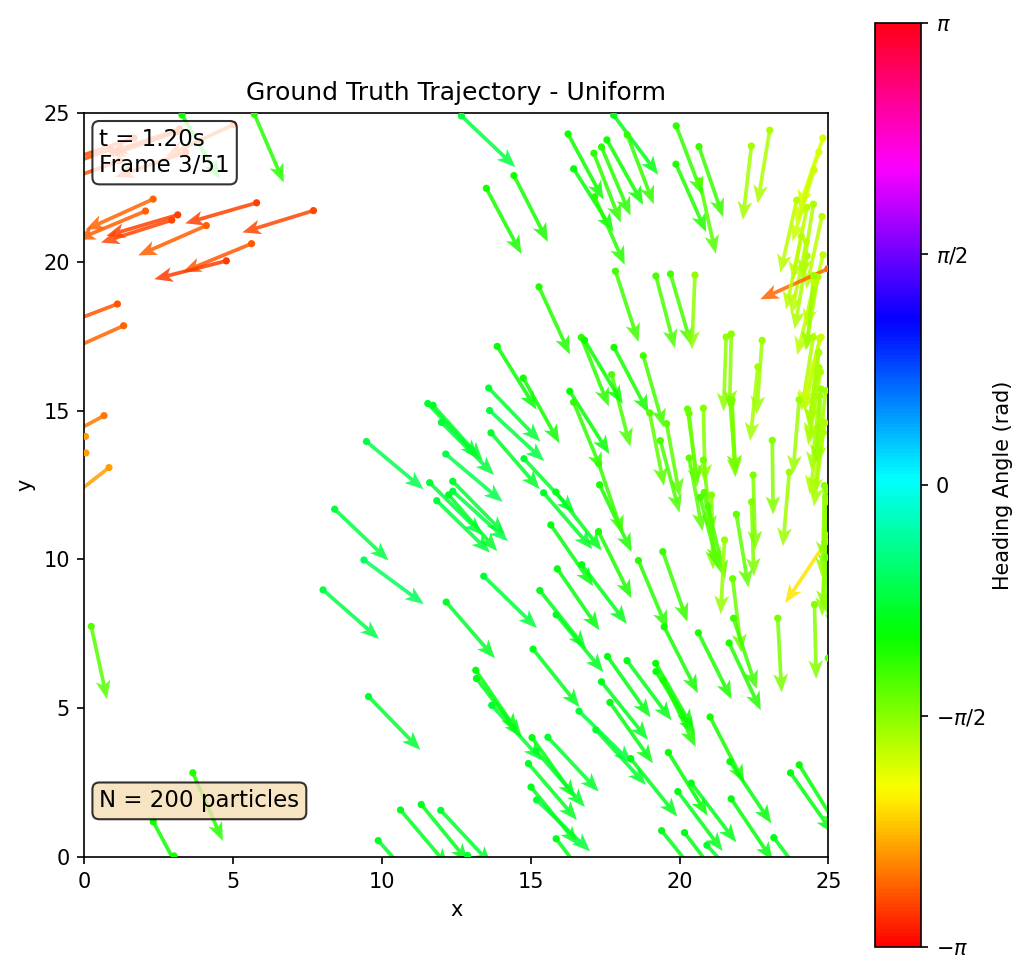
\includegraphics[width=0.33\textwidth]{ch3_experimentation/figures/traj_DYN6_t0.png} &
  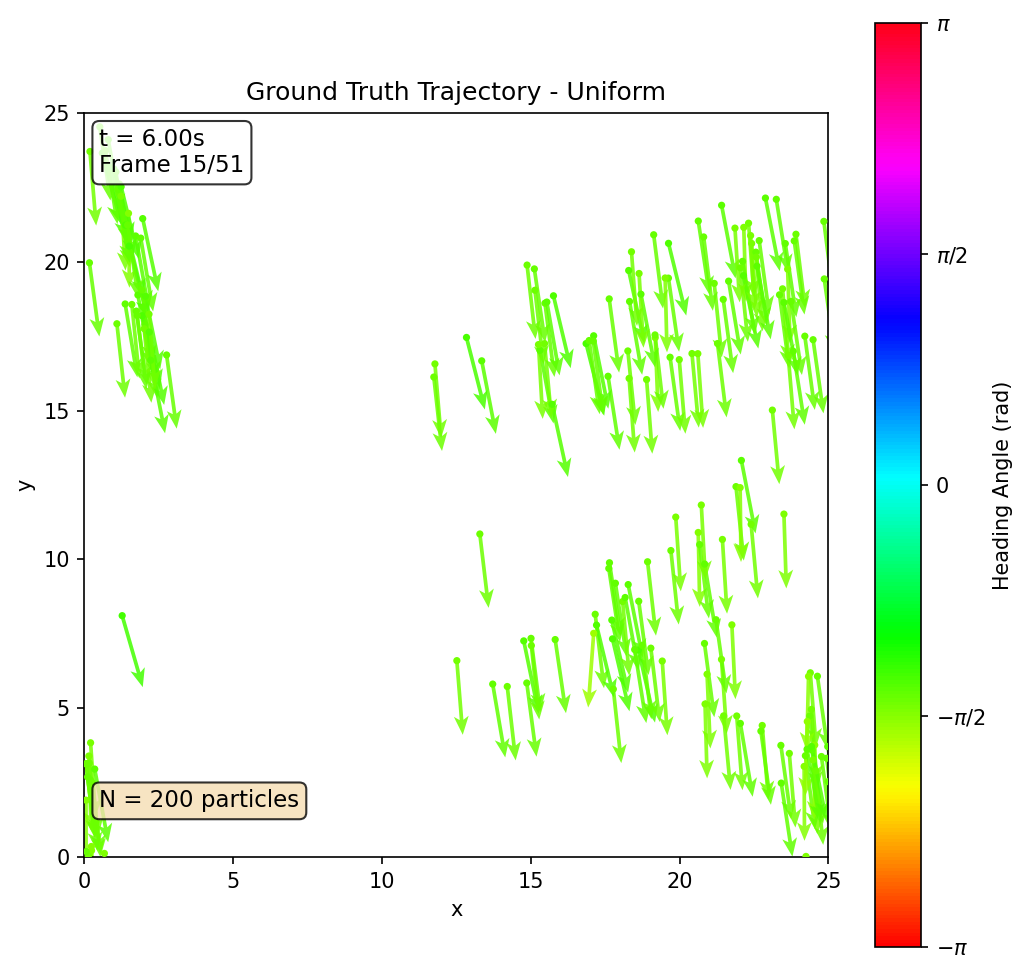
\includegraphics[width=0.33\textwidth]{ch3_experimentation/figures/traj_DYN6_t15.png} &
  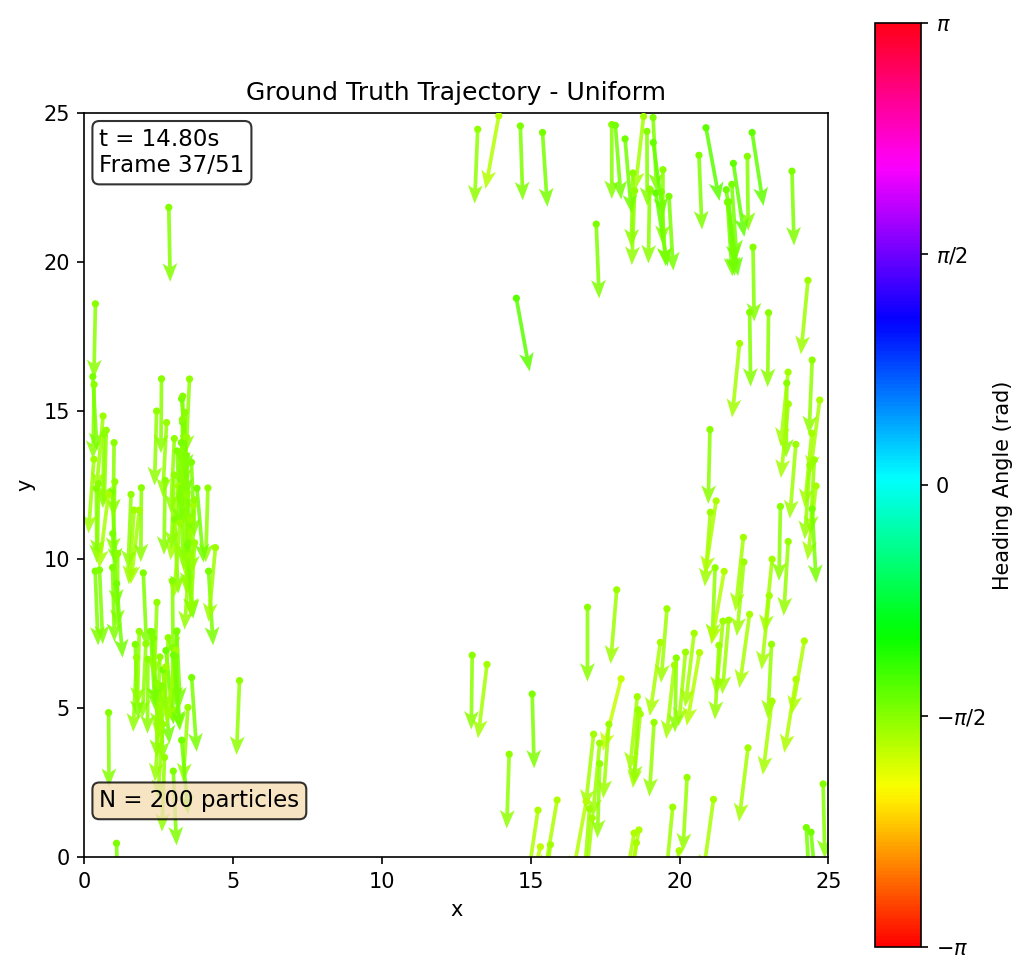
\includegraphics[width=0.33\textwidth]{ch3_experimentation/figures/traj_DYN6_t38.png} \\[-4pt]
  \multicolumn{3}{c}{\small (d) Blackhole VS regime (variable speed --- erratic trajectories)} \\[1pt]

  {\small $t \approx 0$\,s} & {\small $t \approx 6$\,s} & {\small $t \approx 15$\,s}
\end{tabular}}

\caption{Particle trajectories generated by Algorithm~\ref{alg:vicsek} under
  four contrasting parameter regimes, each starting from a uniform initial
  condition.  Arrows indicate heading directions.
  (a)~Gentle crawl: slow drift with gradual clustering from weak Morse
  attraction.
  (b)~Blackhole: rapid collapse into a dense aggregate driven by strong
  attraction ($C_a{=}20$).
  (c)~Pure Vicsek: alignment-only dynamics (no forces) producing coherent
  flocking without spatial aggregation.
  (d)~Blackhole VS: same attraction as (b) but with variable speed;
  stochastic speed fluctuations produce erratic, space-filling trajectories
  that are visually and quantitatively harder to forecast
  (Section~\ref{sec:ch7_shift_dynamics}).}
\label{fig:trajectory_snapshots}
\end{figure}

The Vicsek update therefore defines a nonlinear one-step map on the microscopic state, owing to normalization in the alignment rule, composition of normalization with rotational updates, discontinuous changes in neighbor sets at threshold distance~$R$, and the nonlinear Morse forces combined with directional normalization.  Together, these features produce a high-dimensional, piecewise-smooth dynamical system.

\subsection{Order parameters for emergent behavior}
\label{sec:order_parameters}

These diagnostics are not part of the dynamical model itself; they are regime-level validation observables used to test whether reduced models preserve qualitative collective behavior.
To characterize emergent collective behavior and to validate reduced-order models,
we compute a set of order parameters over time.
Closely related diagnostics for attraction--repulsion systems appear in
\cite{bhaskar2019topology}. Let the center of mass and relative positions be defined by
$x_{\mathrm{cm}}^n := \frac{1}{N}\sum_{i=1}^N x_i^n,
\qquad
r_i^n := x_i^n - x_{\mathrm{cm}}^n$,
Global alignment is quantified by the \emph{polarization} order parameter:
\begin{equation}
\Psi_{\mathrm{pol}}^n
:= \left\|\frac{1}{N}\sum_{i=1}^N \frac{v_i^n}{\|v_i^n\|}\right\|
\in [0,1],
\label{eq:polarization}
\end{equation}
\emph{Angular momentum}\,(milling): measures rotational motion about the center of mass
\begin{equation}
M_{\mathrm{ang}}^n
:= \frac{\left|\sum_{i=1}^N r_i^n \times v_i^n\right|}
{N\,\langle\|r\|\rangle\,\langle\|v\|\rangle},
\qquad
\langle\|r\|\rangle := \frac{1}{N}\sum_{i=1}^N \|r_i^n\|,
\quad
\langle\|v\|\rangle := \frac{1}{N}\sum_{i=1}^N \|v_i^n\|.
\label{eq:angular_momentum}
\end{equation}
The \emph{mean speed} $\langle \|v\| \rangle^n := N^{-1}\sum_{i=1}^N \|v_i^n\|$
serves as a diagnostic for numerical stability.  \emph{Nematic order} (axial alignment)
Axial, head--tail symmetric alignment is quantified by the nematic tensor
\begin{equation}
Q^n := \frac{1}{N}\sum_{i=1}^N \left(n_i^n \otimes n_i^n\right) - \frac{1}{2}I,
\qquad
n_i^n := \frac{v_i^n}{\|v_i^n\|},
\qquad
S^n := \lambda_{\max}(Q^n)
\label{eq:nematic_tensor}
\end{equation}
where $\lambda_{\max}$ denotes the largest eigenvalue. Let $\rho^n \in \mathbb{R}^{N_x\times N_y}$ denote the discretized density field at time $t_n$.
We define the \emph{spatial order} parameter (density heterogeneity) as
\begin{equation}
\mathcal{O}_{\mathrm{spatial}}^n
:= \operatorname{std}\!\left(\rho^n\right)
= \sqrt{\frac{1}{N_x N_y}
\sum_{a,b}\left(\rho_{a,b}^n - \bar\rho^n\right)^2},
\qquad
\bar\rho^n := \frac{1}{N_x N_y}\sum_{a,b}\rho_{a,b}^n.
\label{eq:spatial_order}
\end{equation}
Large values indicate clustered or heterogeneous spatial structure,
while values near zero correspond to near-uniform density distributions.
This diagnostic is used to compare true and predicted density fields in ROM evaluations.

These quantities serve as regime-level validation targets in
Chapters~\ref{ch:rom_results} and~\ref{ch:wsindy_results}.  In particular,
they distinguish failures of transport, clustering, or milling structure
that may not be fully visible from density-space~$R^2$ alone: a forecast
can achieve high pixelwise~$R^2$ yet produce qualitatively wrong
order-parameter trajectories, or conversely preserve the expected
regime-level structure despite moderate density error.


% ==========================================================
% Bibliography notes:
% - vicsek1995: original discrete model with uniform noise, update equations, polarization definition
% - Bhaskar+Ziegelmeier: Morse/D'Orsogna potential + order parameter formulas used in our extended regime analysis
% ==========================================================

\section{Kernel density estimation and coarse-graining scale}
\label{subsec:kde}

KDE is not simply a visualisation convenience: it defines the macroscopic field on which both the EF-ROM and WSINDy branches operate.  Because both branches consume the same KDE output, the comparison between them is fair, but both inherit the same upstream smoothing bias, and every
PDE coefficient recovered in later stages must be interpreted relative
to the chosen bandwidth.

Following the equation-free framework of~\cite{alvarez2025eqfree}, the KDE step serves as a coarse-graining operator that maps discrete positions $\{x_i(t)\}_{i=1}^N$ to a smooth \emph{number density} field $\rho(\cdot,t)$.
In continuous form, we define
\begin{equation}
\rho(x,t)
=
\sum_{i=1}^N K_h\!\bigl(x-x_i(t)\bigr),
\label{eq:kde_def}
\end{equation}
where $K_h$ is a smooth, nonnegative kernel with bandwidth $\sigma$ specified in grid-cell units (so the physical smoothing length is $h=\sigma\,\Delta x$) controlling the smoothing level and normalized so that
$\int_{\mathbb{R}^2} K_h(z)\,dz = 1$.
With this convention, $\rho$ has units of \emph{particles per unit area} and satisfies the mass constraint
$\int_\Omega \rho(x,t)\,dx = N$ (up to discretization), which is essential for subsequent POD-based compression and mass-preserving lifting.

We use an isotropic Gaussian kernel,
\begin{equation}
K_h(z)
=
\frac{1}{2\pi h^2}
\exp\!\left(-\frac{\|z\|^2}{2h^2}\right),
\label{eq:gaussian_kernel}
\end{equation}
which provides smooth coarse-graining appropriate for periodic rectangular domains.

\begin{remark}[Histogram plus Gaussian smoothing approximates gridded Gaussian KDE]
\label{claim:histogram_kde}
Let $\tilde\rho(\cdot,t)$ be the piecewise-constant histogram number density on a uniform grid with spacings
$\Delta x = L_x/n_x$ and $\Delta y = L_y/n_y$.
Let $G_\sigma$ denote the discrete Gaussian convolution operator (standard deviation $\sigma$ in \emph{grid-cell units}) applied to the gridded field $\tilde\rho$.
If the grid is square ($\Delta x=\Delta y$) and the same $\sigma$ is used in both axes, then the smoothed histogram
\begin{equation}
\rho(\cdot,t) \;=\; G_\sigma * \tilde\rho(\cdot,t)
\label{eq:smoothed_histogram}
\end{equation}
approximates the \emph{cell-averaged} continuous Gaussian KDE \eqref{eq:kde_def} with physical bandwidth $h=\sigma\,\Delta x$.
This follows from standard properties of Gaussian convolution; for foundational KDE theory see, e.g.,~\cite{wasserman2006all}.
\end{remark}

\begin{remark}[Mass conservation in periodic domains]
\label{rem:kde_mass}
For periodic boundary conditions, Gaussian smoothing with wrapped boundaries
preserves discrete mass: $\sum_{a,b} (G_\sigma * \tilde\rho)_{ab} = \sum_{a,b} \tilde\rho_{ab}$, since the discrete Gaussian filter weights sum to~$1$. The total mass $M(t) := \sum_{a,b} \rho_{ab}(t)\,\Delta x\,\Delta y$ therefore equals $N$ up to floating-point error.
\end{remark}

The full pseudocode is given in Algorithm~\ref{alg:kde_hist_gauss}
(Appendix~\ref{app:detailed_algorithms}).

\emph{Implementation details:} We specify the bandwidth $\sigma$ in grid-cell units, so the physical smoothing length is $h=\sigma\,\Delta x$ (for a square grid $\Delta x=\Delta y$).
All experiments use $\sigma=5.0$ grid cells (so $h=5\,\Delta x$) with $n_x=n_y=64$.
We record metadata (bandwidth, grid resolution, domain size, boundary condition) alongside the resulting density movie $\rho(t)\in\mathbb{R}^{T\times n_y\times n_x}$, which serves as input to POD-based compression and subsequent reduced-order modeling.

The bandwidth is part of the coarse-grained model, not
merely a numerical tuning parameter: it sets the spatial scale at which
the macroscopic field is defined, and thereby determines which
microscopic structures are visible to the regression stage.  Smaller
bandwidths retain more localised structure but increase variance and may
worsen derivative-sensitive tasks such as weak-form regression; larger
bandwidths reduce noise but risk erasing clustering and nonlocal
interaction signatures that the WSINDy library is designed to detect.
The chosen value $\sigma=5$ therefore
reflects a trade-off between preserving emergent spatial structure and
obtaining stable reduced and weak-form models; at this scale, short-range interaction structure (sub-five-cell features) may be unrecoverable, even if longer-range alignment and attraction signatures remain visible.  No systematic bandwidth
sensitivity study was performed; the values used here were selected
empirically and held fixed across all regimes.  All recovered PDE
coefficients, and the ROM forecast quality, are conditional on this
fixed coarse-graining choice.

\subsection{Multi-field coarse-graining}
\label{sec:multifield_cg}

Beyond the scalar density $\rho$, the multi-field WSINDy formulation (Chapter~\ref{ch:wsindy_methodology}) requires
two additional coarse-grained fields and, optionally, a nonlocal interaction field.
All three are computed using the same
histogram-plus-Gaussian-smoothing approach as the density KDE above.

\paragraph{Polarisation flux fields.}
The velocity-weighted \emph{polarisation flux} fields $p_x,p_y$
are defined by replacing the unit weight in~\eqref{eq:kde_def} with the
corresponding velocity component:
\begin{equation}
p_\alpha(x,t)
=
\sum_{i=1}^N K_h\!\bigl(x-x_i(t)\bigr)\,v_{i,\alpha}(t),
\qquad \alpha\in\{x,y\},
\label{eq:flux_kde}
\end{equation}
where $K_h$ is the same Gaussian kernel used for $\rho$.
In practice, velocity-weighted counts are deposited
into a 2-D histogram and smoothed with the same Gaussian kernel and
periodic boundary handling used for the density, yielding
$p_x,p_y\in\mathbb{R}^{T\times n_y\times n_x}$.

\paragraph{Morse potential field.}
The Morse interaction potential field $\Phi$ is the convolution
of the density with the radial Morse kernel
$W(r) = -C_r\,e^{-r/\ell_r} + C_a\,e^{-r/\ell_a}$:
\begin{equation}
\Phi(x,t)
=
(W * \rho)(x,t)
=
\mathcal{F}^{-1}\!\bigl[\hat W \cdot \hat\rho\bigr](x,t),
\label{eq:morse_potential_field}
\end{equation}
evaluated efficiently via 2-D FFT convolution.
The combined field set $(\rho, p_x, p_y)$---together with their spatial
derivatives and, when forces are active, $\Phi$---forms the input to the
weak-form PDE library constructed in Chapter~8.

These auxiliary fields are introduced because the macroscopic flux is not
expected to close as a function of density alone.  The polarization fields
encode directional alignment information that is lost by scalar KDE, while
the Morse potential provides a nonlocal summary of attraction--repulsion
interactions.  In the WSINDy branch, these fields are treated as
coarse observables supporting a coupled closure model, rather than as exact
mean-field state variables derived from first principles.

\paragraph{Summary.}
The microscopic Vicsek--Morse simulator generates the trajectory data
from which all results in this thesis derive.  KDE with a fixed Gaussian
bandwidth converts those trajectories into shared macroscopic fields
$(\rho, p_x, p_y, \Phi)$ on a periodic grid.  The chosen bandwidth
fixes the coarse-graining scale; both the EF-ROM forecast quality and
the WSINDy-recovered PDE coefficients must be interpreted relative to
that field representation.  This shared upstream ensures a fair
comparison between the two branches, while also implying that any
smoothing bias propagates to every subsequent result.
